\paragraph{Definition}
A continuous variable $X$ is said have a Chi-Square distribution with
$r$ degrees of freedom if its probability density function is of the form
$$
f(x;r)=
\left\{
\begin{array}{ll}
\dfrac{1}{\Gamma\left(\frac{r}{2}\right)^{2^{\frac{r}{2}}}}x^{\frac{r}{2}-1}e^{-\frac{x}{2}} & \mbox{if } 0 \leq x\leq \infty \\
0 & \mbox{otherwise}
\end{array}
\right.
$$
Recall that a gamma distribution reduces to Chi-Square distribution if 
$\alpha = \frac{r}{2}$ and $\theta = 2$.
\begin{figure}[H]
	\begin{center}
		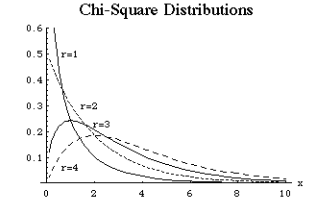
\includegraphics[width=\textwidth]{./chaps/23sec/images/1chi_square.png}
	\end{center}
	\caption{If $r\rightarrow\infty$ then chi-square distribution
	tends to normal distribution}
	\label{fig:23sec_chiSquared}
\end{figure}

\paragraph{Properties}
\subparagraph{Population}
If $X\hookrightarrow N(\mu, \sigma^{2}) \text{, then }\left( \frac{X-\mu}{\sigma} \right)^{2}\hookrightarrow\chi^{2}(1)$
\subparagraph{Sample} If $X\hookrightarrow N(\mu,\sigma^{2})\text{ and }\prth{X}{i}{1}{n}$ is a random sample from $X$, then:\\
$$ \su{{i=1}}{n}\left( \dfrac{X_{i}-\mu}{\sigma} \right)^{2}\hookrightarrow\chi^{2}(n)$$
\subparagraph{Sample variance} If $X\hookrightarrow N(\mu,\sigma^{2})\text{ and }\prth{X}{i}{1}{n}$ is a random sample from $X$, then:\\
$$ \dfrac{(n-1)S^{2}}{\sigma^{2}}\hookrightarrow\chi^{2}(n-1)$$
\subparagraph{Gamma} IF $X\hookrightarrow \gamma(\theta,\alpha)$, then:
$$ \dfrac{2}{\theta}\hookrightarrow\chi^{2}(2\alpha)$$
